% Exercise ID: MAT_P4FUNCOE_4FIN_TRH_004
% Exercise ID: MAT_P4FUNCOE_4FIN_TRH_004
% Module: MÓDULO P4 - Funções | Concept: Função Inversa | Type: Teste da Reta Horizontal
% Difficulty: 2/5 (Fácil) | Type: desenvolvimento
% Points: 10 | Time: 10 min
% Tags: inversa, injetividade, teste_reta_horizontal, grafico
% Author: Professor | Date: 2025-11-18
% Status: active
% Description: Determinar quais funções são invertíveis usando teste da reta horizontal

\exercicio
Considere as funções representadas nas figuras seguintes:

\begin{figure}[H]
\centering
\begin{minipage}{0.45\textwidth}
\centering
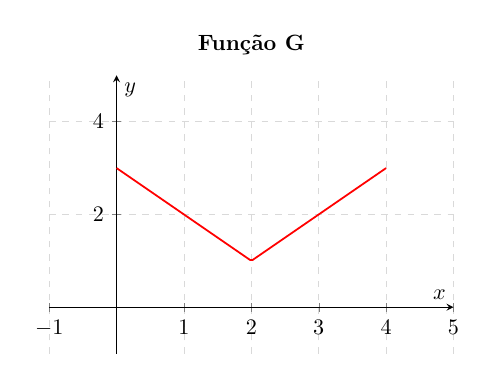
\begin{tikzpicture}[scale=0.8]
    \begin{axis}[
        axis lines = middle,
        xlabel = $x$,
        ylabel = $y$,
        xmin = -1, xmax = 5,
        ymin = -1, ymax = 5,
        grid = major,
        grid style = {dashed, gray!30},
        width = 8cm,
        height = 6cm,
        title = {Função G},
        title style = {font=\bfseries},
    ]
    \addplot[domain=0:4, samples=100, thick, red] {abs(x-2)+1};
    \end{axis}
\end{tikzpicture}
\end{minipage}
\hfill
\begin{minipage}{0.45\textwidth}
\centering
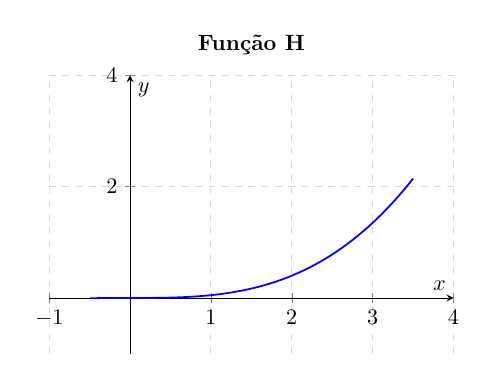
\begin{tikzpicture}[scale=0.8]
    \begin{axis}[
        axis lines = middle,
        xlabel = $x$,
        ylabel = $y$,
        xmin = -1, xmax = 4,
        ymin = -1, ymax = 4,
        grid = major,
        grid style = {dashed, gray!30},
        width = 8cm,
        height = 6cm,
        title = {Função H},
        title style = {font=\bfseries},
    ]
    \addplot[domain=-0.5:3.5, samples=100, thick, blue] {x^(3)/20};
    \end{axis}
\end{tikzpicture}
\end{minipage}
\end{figure}



Quais das duas funções são invertíveis (isto é, cuja inversa também é uma função)? Justifique usando o teste da reta horizontal.

\vspace{3cm}